\documentclass{article}
\usepackage[pdftex]{graphicx}
\usepackage{amsmath}
\usepackage{verbatim}
\usepackage{enumerate}
\author{Michael Anderson}
\title{Takehome Final}
\begin{document}
\maketitle
\center{CS533}
\center{Prof. Fern}\\
\flushleft
\newpage

\section{}
Imagine a k-order MDP in which all states have at most one parent state. In
other words, for all $s'$ that are states in the MDP, there exists at most one
$s$ such that $T(s,a,s') > 0$. Such a k-order MDP would be directly
convertible to a first-order MDP, because each state would have one
possible vector of ancestor states.

\vspace{1em}

However, in a normal k-order MDP where states can have multiple parents,
a state could have a number of different ancestor vectors, and that information
is not accounted for in first-order MDP.

\vspace{1em}

So, to convert a k-order MDP $M$ to a first-order MDP $M'$, traverse M cloning
states, actions, rewards, and transitions over to $M'$ exactly, except
whenever a state $s$ is found with multiple parents. In that case make a set of 
states in $S'$ to represent such an $s'$ in $S$, $\{s'_1,s'_2,...,s'_k\}$,
one state for each of the $k$ parents to transition to. Also
duplicate all of the descendants of $s'$, so that {$s_1,s_2,...,s_k$} each have 
their
own copy. Finally, when copies of descendants are made in this way, check to
see if they can be merged back together farther down the tree when they have the
same ancestor vectors again (see picture).

\vspace{1em}

The handling of $A'$, $R'$, and $T'$ are straightforward. For states without
multiple
parents, they are identical to $A$, $R$, and $T$. But supposing that for some
state
$s'$ in S there exists multiple $s$ such that $s$ is in $S$ and $T(s,a,s') > 0$,
then for each such $s$ with a corresponding $a$ that reaches $s'$, make $a$ a
member of $A'$ and make $T'(s,a,s_i) = T(s,a,s')$. For the rewards, make
$R'(s_i) = R(s')$.

\vspace{1em}

Below is an example of part of a 3-order MDP $M$ and the corresponding part of
its equivalent first-order MDP $M'$. This MDP is deterministic for simplicity,
but without loss of generality.
States are labeled 1 through 9 in $M$, and
in $M'$ states are labeled by their grandfather, their father, and then the
state themselves. Notice that since 5 and 6 have two parents, they are each
expanded into two states in $M'$. 7 is expanded into four states, because it
has four combinations of grandfather/father pairs. 8 only has two such
combinations and 9 only has one, so we see in the picture an example of the
merging of descendant states mentioned above. 

\newpage

\begin{center}

$M$
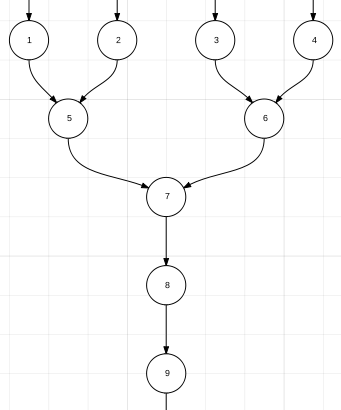
\includegraphics[scale=0.85]{M.png}

\vspace{5em}

$M'$
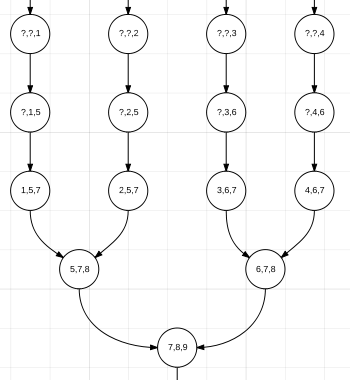
\includegraphics[scale=0.85]{M_prime.png}

\end{center}


\section{}
Let $g(\theta_1,...,\theta_n) = e^{Q_{\theta}(s,a)}$ and $h(\theta_1,...,
\theta_n) = \sum_{a'} e^{Q_{\theta}(s,a')}$. Then $\pi_{\theta}(s,a) = g/h$
and we want to compute:

\[
\frac{\partial log(\frac{g}{h})}{\partial \theta_i}
\]

Using $'$ as shorthand for the partial derivative in question, and applying the
chain rule and quotient rule gives:

\[
\frac{\partial log(\frac{g}{h})}{\partial \theta_i} = 
\frac{h}{g} \times \frac{\partial \frac{g}{h}}{\partial \theta_i} = 
\frac{h}{g} \times \frac{g'h-gh'}{h^2} = \frac{g'}{g} - \frac{h'}{h}
\]

Need to apply the chain rule to differentiate g, and the hard part is
differentiating the $Q_\theta(s,a)$ portion. Since all of the parts of the 
summation that
defines $Q_{\pi}$ are constant or held constant excepting $\theta_i$, 
$Q'_{\pi}(s,a)$ is simply $f_i(s,a)$. So we get:

\[
g' = \frac{\partial e^{Q_{\theta}(s,a)}}{\partial \theta_i} =
f_i(s,a) e^{Q_{\theta}(s,a)}
\]

Differentiating h is similar:

\[
h' = \frac{\partial \sum_{a'}e^{Q_{\theta}(s,a')}}{\partial \theta_i} = 
\sum_{a'} \frac{\partial e^{Q_{\theta}(s,a')}}{\partial \theta_i} =
\sum_{a'} f_i(s,a') e^{Q_{\theta}(s,a')}
\]

Now we are ready to finish:

\[
\frac{\partial log(\pi_{\theta}(s,a))}{\partial \theta_i} = 
\frac{g'}{g} - \frac{h'}{h} =
\]

\vspace{6pt}

\[
\frac{f_i(s,a) e^{Q_{\theta}(s,a)}}{e^{Q_{\theta}(s,a)}} - 
\frac{\sum_{a'} f_i(s,a') e^{Q_{\theta}(s,a')}}{\sum_{a'} e^{Q_{\theta}(s,a')}}
=
\]

\vspace{6pt}

\[
\frac{f_i(s,a) e^{Q_{\theta}(s,a)}}{e^{Q_{\theta}(s,a)}} - 
\sum_{a'} \frac{e^{Q_{\theta}(s,a')}}{\sum_{a'} e^{Q_{\theta}(s,a')}} f_i(s,a') 
= 
\]

\vspace{6pt}

\[
f_i(s,a) - \sum_{a'}\pi_{\theta}(s,a')f_i(s,a')
\]

\newpage


\section{}

Assume the worst case, which is that the maximum reward $R_{max}$ is obtained
at each level of the tree. Then at search depth h, the reward is
$\beta^h R_{max}$, because $R_{max}$ is discounted by a factor of $\beta$ at
each level. The infinite horizon reward becomes an easily simplifiable
geometric series:

\[
Q_\pi(s,a) = \sum_{i = 1}^{\infty} \beta^i R_{max} =
\frac{1}{1-\beta}R_{max}
\]

The finite horizon reward then, for a horizon of $h$, is

\[
Q_\pi(s,a,h) = \sum_{i = 1}^{h} \beta^i R_{max} = 
\frac{1-\beta^h}{1-\beta}R_{max}
\]

Since this is the worst case, the difference between $Q_\pi(s,a)$ and
$Q_\pi(s,a,h)$ is maximized by:

\[
\frac{1}{1-\beta}R_{max} - \frac{1-\beta^h}{1-\beta}R_{max} =
\frac{\beta^h}{1-\beta}R_{max}
\]

\newpage


\section{}
\begin{enumerate}[(a)]
\item
\emph{No}, it is definitely not complete. If a proposition in state
$s_i$ that is not deleted by $a_i$ does not persist to $s_{i+1}$, then the
algorithm ends up with a restricted view of the environment, and may lose
information that it needs to find a route to the goal. Consider the following
planning graph:

\begin{center}

\includegraphics{planning.png}

\end{center}

In s0 prop1 and prop2 are asserted, in a0 action1 can be taken to add 
prop3 and delete its precondition prop1, then in s1 action2
(with preconditions prop3 and prop2) can be taken to reach propGoal, which we
will assume is the only proposition of the goal state.

\vspace{1em}

In this scenario, it is only possible to reach the goal if prop2 persists from
s0 to s1. If that persistence action was not there, then GraphPlan would
fail to find a path to the goal state, and is therefore incomplete.

\item
\emph{No}, it is definitely not sound. The purpose of computing mutex
relations is not only to prune the search tree, making GraphPlan
more efficient, but also to ensure that it produces valid layered plans. For
example, suppose at some level we have the necessary preconditions to take
either of two actions, but one action deletes
a precondition of the other action. Using mutexes will rule out these two
actions as not valid in the same layer, but without using mutexes GraphPlan
could place them in the same layer. Since one deletes a precondition of the
other, the order that the actions were taken in would be significant, and a plan
putting them in the same layer would be unsound.

\end{enumerate}

\newpage


\section{}
\begin{enumerate}[(a)]
\item
Since the total error is at worst the sum of the errors introduced by a finite
horizon $h$ and a finite $w$, i.e. $\epsilon_h + \epsilon_w \le \epsilon$, we
can set $h$ and $w$ to get their own half of $\epsilon$. So
$\epsilon_h=\epsilon_w = \epsilon/2$.

\vspace{1em}

The error introduced by a finite $h$ was derived in Question 3:

\[
\frac{\beta^h}{1-\beta}R_{max} \le \epsilon_h \Longrightarrow
\]
\[
h = log_{\beta}(\frac{(\epsilon /2)(1-\beta)}{R_{max}})
\]

It is given that the Chernoff bound bounds the error introduced by a finite $w$.
So choose w based on that equation:

\[
w = (\frac{R_{max}}{e/2})^2 \times log(\frac{1}{\delta'})
\]

\item
Now the chance that any individual QEstimate is wrong is $\delta '$, from which
we can calculate the chance $\delta$ that any of $|A|$ of them are wrong, and
then choose a $\delta '$. $\delta$ is the opposite of all of them being right,
which are $|A|$ independent events, so:

\[
\delta = 1-(1-\delta')^{|A|} \Longrightarrow
\]
\[
\delta' = 1 - \sqrt[|A|]{1-\delta}
\]

Now, if $Q_1(s) - Q_2(s) = \Delta(s)$, then if the estimate of $Q_1(s)$ is
$>\Delta(s)/2$ too high, and the estimate of $Q_2(s)$ is $>\Delta(s)/2$
too low, then $Q_2$ will incorrectly appear better than $Q_1(s)$, so finally
we have:

\[
\epsilon = \frac{\Delta(s)}{2}
\]

\end{enumerate}

\end{document}
